\section*{Best vs Pretty models}

We provide qualitative comparison between the our models trained with \emph{best} and \emph{pretty} configurations in~\figref{best_vs_pretty}.
The \emph{best} configuration refers to our model trained without edge regularization while \emph{pretty} refers to the model trained with the regularization (\subsecref{experimental_setup}).
We observe that without the regularization we get higher score on our evaluation metrics but get degenerate meshes with self-intersections and irregularly sized faces.

\begin{figure*}[h]
    \begin{center}
        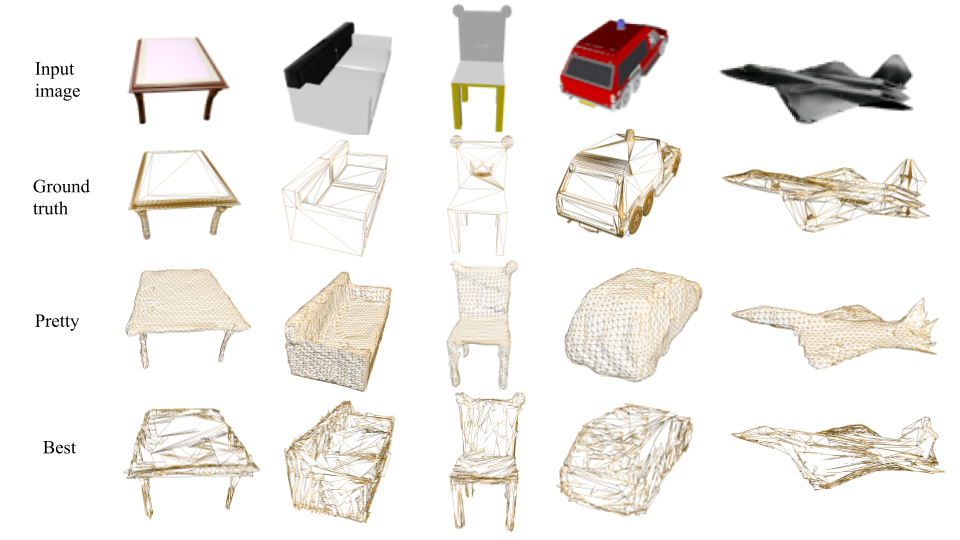
\includegraphics[width=\linewidth]{imgs/best_vs_pretty.png}
    \end{center}
    \vspace{-4mm}
        \caption{Qualitative evaluation: best vs pretty wireframe models. The best models while being preferred by the evaluation metrics lead to degenerate meshes, with irregularly sized faces and self-intersections}
        \vspace{-4mm}
        \label{fig:best_vs_pretty}
\end{figure*}

\newpage
\section*{Failure Cases}

Some failure cases of our model (with pretty setting) are shown in~\figref{failure_cases}.
% We notice that our system can still struggle with shapes with very complex topology.
We notice that the rough topology of the mesh is recovered while we failed to reconstruct the fine topology.
We can regard the recovery from wrong initial topology as a promising future work.

\begin{figure*}[h!]
    \begin{center}
        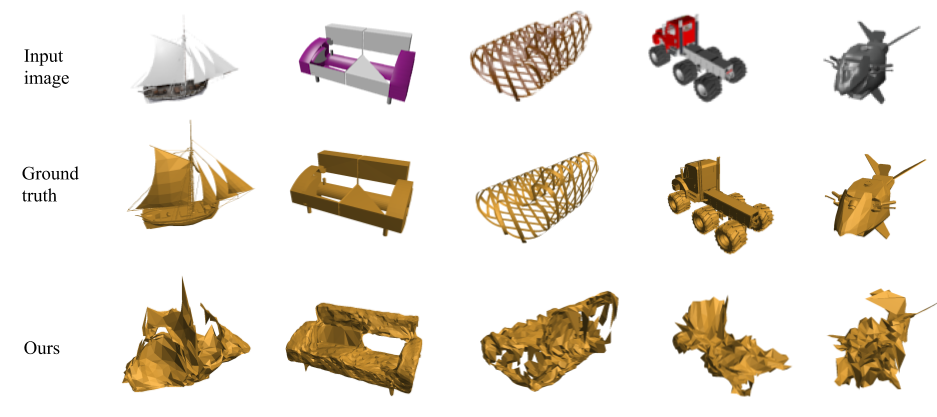
\includegraphics[width=\linewidth]{imgs/failure_cases.png}
    \end{center}
    \vspace{-4mm}
        % \caption{Failure Cases. Our system can still struggle to reconstruct shapes with very complex topology.}
        \caption{Failure Cases. Our system can struggle to roughly reconstruct shapes with very complex topology while some fine topology of the mesh is missing.}
        \vspace{-4mm}
        \label{fig:failure_cases}
\end{figure*}
